\documentclass[12pt]{article}
\usepackage[spanish]{babel}
\usepackage{makeidx}
\usepackage[margin=1in]{geometry}  % set the margins to 1in on all sides
\usepackage{graphicx}              % to include figures
\usepackage{amsmath}               % great math stuff
\usepackage{amsfonts}              % for blackboard bold, etc
\usepackage{amsthm}                % better theorem environments
\usepackage{makeidx}               % index
\usepackage[utf8]{inputenc}        % now we have tildes!
\usepackage{wrapfig}               % images
\usepackage{listings}              % Unordered lists
\usepackage{hyperref}              % hyperlinks
\usepackage{xcolor}                % to colorize font
\usepackage{blindtext}             % to colorize font

\makeindex

\begin{document}

\begin{titlepage}

\newcommand{\HRule}{\rule{\linewidth}{0.5mm}} % Defines a new command for the horizontal lines, change thickness here

\center % Center everything on the page

%----------------------------------------------------------------------------------------
%	LOGO SECTION
%----------------------------------------------------------------------------------------

\textsc{\LARGE Universidad Carlos III de Madrid}\\[1.2cm] % Name of your university/college

%----------------------------------------------------------------------------------------
%	HEADING SECTIONS
%----------------------------------------------------------------------------------------


\includegraphics[width=9cm]{Logo}\\[1.2cm] % Include a department/university logo - this will require the graphicx package

\textsc{\Large Aprendizaje Automático}\\[0.5cm] % Major heading such as course name
\textsc{\large Grado en Ingeniería Informática}\\[0.6cm] % Minor heading such as course title
\textsc{\large Grupo 83}\\[0.5cm]

%----------------------------------------------------------------------------------------
%	TITLE SECTION
%----------------------------------------------------------------------------------------

\HRule \\[0.7cm]
{ \huge \bfseries Práctica 2: Aprendizaje basado en instancias}\\[0.4cm] % Title of your document
\HRule \\[0.7cm]

%----------------------------------------------------------------------------------------
%	AUTHOR SECTION
%----------------------------------------------------------------------------------------

\emph{Autores:}\\
Daniel \textsc{Medina García}\\ % Your name
Alejandro \textsc{Rodríguez Salamanca}\\[1.1cm] % Your name

%----------------------------------------------------------------------------------------
%	DATE SECTION
%----------------------------------------------------------------------------------------

{\large \today}\\ % Date, change the \today to a set date if you want to be precise

%----------------------------------------------------------------------------------------

\vfill % Fill the rest of the page with whitespace

\end{titlepage}

\tableofcontents

\newpage
\thispagestyle{empty}
\clearpage
\vspace*{\fill}
\begin{center}
    \begin{minipage}{\textwidth}
        \begin{center}
            \section*{Introducción}
            El presente documento contiene la memoria del trabajo realizado para esta segunda práctica de Aprendizaje Automático. En ella, el equipo ha utilizado el aprendizaje basado en instancias, haciendo uso de la técnica de \emph{clustering} para poder implementar funciones de afinidad y agilizar así la clasificación. Continuamos así nuestra introducción al aprendizaje no supervisado, en oposición al aprendizaje supervisado visto en ejercicios anteriores.
        \end{center}
    \end{minipage}
\end{center}
\vfill

\newpage
\section{Recogida de información}

% Descripción de las variables que representan el estado, así como su rango de valores.

Tomamos como base la toma de datos de la anterior práctica, para construir sobre ella ligeras mejoras que en nuestra opinión optimizaban la información almacenada. Así, los siguientes datos fueron recopilados en tiempo de ejecución:

\begin{itemize}
    \item \texttt{score} : atributo numérico que contiene la puntuación instantánea. Su rango es en principio ilimitado, si bien oscila en nuestros datos desde -30 hasta 600 jugando con el agente de teclado. Cabe esperar que los resultados obtenidos con el agente automático no sean tan buenos, por lo que consideramos razonable generalizar y considerar su rango de entre menos 1000 y 1000. Si bien esa cota superior es real (cada fantasma comido aporta 250 puntos y esta práctica usa tan solo 4 fantasmas), la inferior es un margen holgado en base a nuestros datos (para llegar a una puntuación tan baja el agente debería de no comer ningún fantasma y estar 1000 turnos sin comer ninguno, y esta situación tiene probabilidades despreciables de aparecer).
    \item \texttt{ghosts-living} : atributo numérico que lleva la cuenta de los fantasmas que quedan vivos en el momento actual. Su valor oscila entre 1 (sólo queda un fantasma por cazar) y 4 (situación inicial).
    \item \texttt{distance-ghost}$_{i}$ : cuatro atributos numéricos que hacen de vector de distancias a los respectivos fantasmas en este turno.
    \item \texttt{prev-distance-ghost}$_{i}$ : cuatro atributos numéricos que expanden la información desde el turno anterior para evaluar el acercamiento o distanciamiento a los fantasmas. Todas las distancias tienen como mínimo 1 y la diagonal del tablero como máximo.
    \item \texttt{pos\textless axis\textgreater} : coordenadas de PacMan, en forma de número entero. Sus valores se encuentran dentro del rango de los ejes \emph{X} e \emph{Y} del mapa de juego.
    \item \texttt{direction} : atributo enumerado que indica el anterior movimiento de PacMan, comprendido entre los cinco posibles valores \emph{North, South, East, West} y \emph {Stop}.
    \item \texttt{wall-\textless direction\textgreater} : 4 atributos enumerados en forma booleano que indican si hay o no un muro en las posiciones contiguas a PacMan.
    \item \texttt{move} : Acción que toma el agente en el turno actual, con posibles valores \emph{North, South, East, West} y \emph {Stop}, si bien esperamos que esta última no sea tomada nunca.
    \item En continuación de la parte de predicción de la \emph{Práctica 1}, almacenamos seguidamente todos los atributos mencionados hasta ahora a cuatro turnos vista. Estos atributos pueden verse en el archivo como \textless atributo\textgreater N, indicando que es el atributo del turno futuro.
    \item \texttt{fx} : valor de la función de evaluación, que explicaremos más adelante.
\end{itemize}

\section{Clustering}

% Descripción y justificación de los algoritmos utilizados para el proceso de \emph{clustering}.

Tras probar todos los diferentes algoritmos de \emph{clustering} ofrecidos por \emph{Weka}, hicimos un primer filtro con aquellos que nos daban un número manejable de \emph{clusters} (o se podía configurar dicho número) para evitar aquellos que generaban demasiados (menos de un 5\% de pertenencia) o insuficientes (menos de 4). Esta primera selección nos dejó con \emph{Cobweb}, \emph{EM}, \emph{FarthestFirst} y \emph{SimpleKMeans}. Comparando los algoritmos, buscamos dos propiedades: equilibrio entre los \emph{clusters} y ``estabilidad'' entre ejecuciones al modificar los parámetros (i.e. semilla u otras constantes). Esta comparativa nos hizo decantarnos por \emph{SimpleKMeans} y \emph{EM}, pues los porcentajes de pertenencia a cada \emph{cluster} eran más parecidos entre sí y distintas semillas resultaban en \emph{clusters} de dimensiones similares.

Si bien los resultados eran parecidos entre estos dos algoritmos, el elevado coste en tiempo para elaborar el \emph{clustering} con \emph{EM} nos hizo decantarnos por \emph{SimpleKMeans}. Mostramos a continuación la justificación de nuestra decisión, donde observamos el equilibrio conseguido con este algorimo de \emph{clustering} y su estabilidad ante el cambio de la semilla. Cabe destacar que con los otros algoritmos encontramos variaciones muy superiores (e.g. entre 11 y 17\% con \emph{FarthestFirst}, alcanzando el 15\% con \emph{Cobweb}), alejadas de la media de 6\% obtenida con \emph{SimpleKMeans}.

\begin{center}
    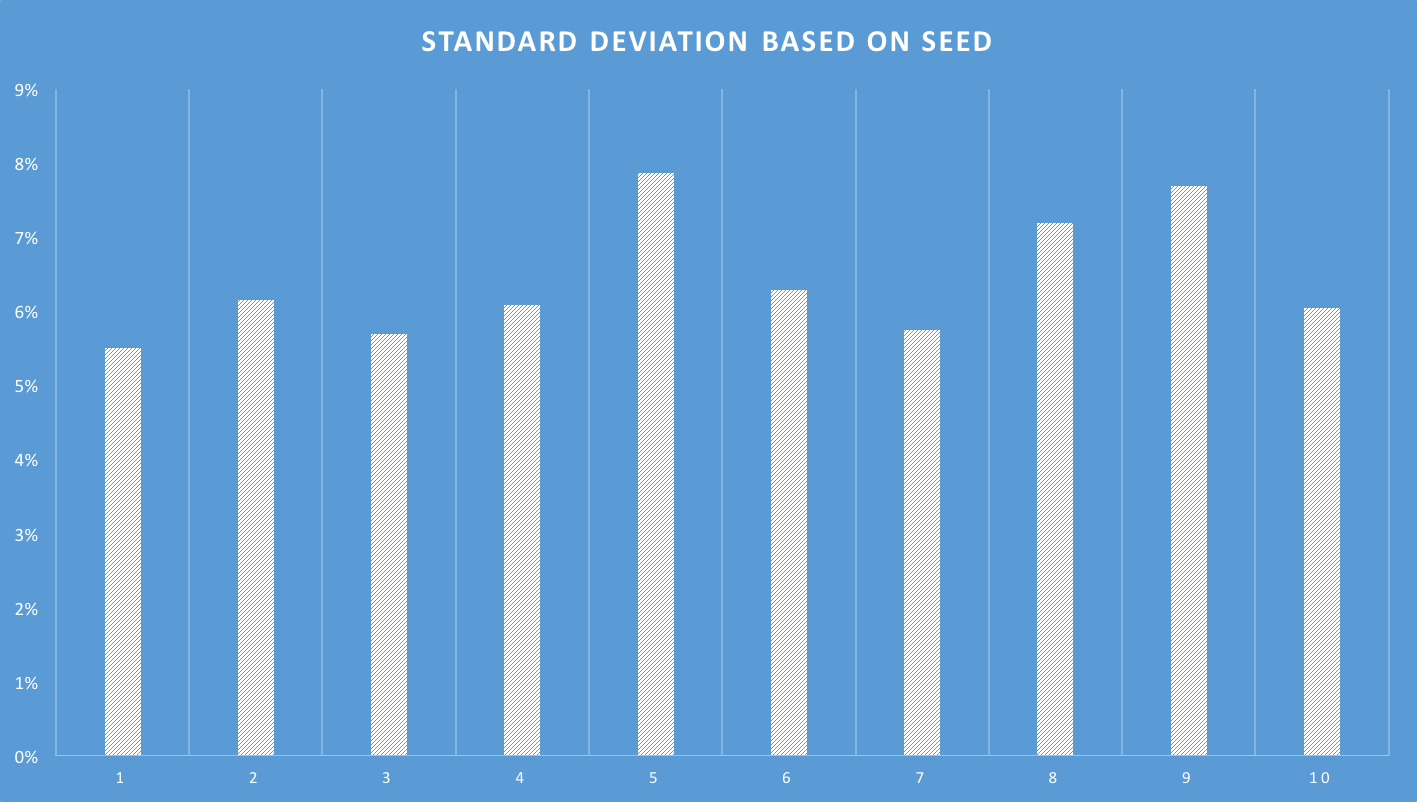
\includegraphics[width=15cm]{stdff}
\end{center}

% Descripción de cualquier tratamiento sobre los datos que se lleve a cabo y de todos los pasos realizados.

Para potenciar la eficacia de la clusterización, probamos a normalizar los datos. Sin embargo, los resultados obtenidos fueron los mismos. Como la normalización de los datos dificultaba la inclusión de nuevas instancias desde el wrapper de \emph{Weka} para \texttt{Python} a un fichero ya normalizado, decidimos excluir este y otros filtros de preproceso de los datos. Para determinar si los movimientos tomados habían sido o no buenos, elaboramos una función cuyo incremento entre turnos supondría un rendimiento productivo. Esta función, que consta de tres sumandos con un coeficiente a modo de peso para evaluar distintos aspectos del agente, nos ayudará a descartar las instancias que no consideremos que ayuden para clusterizar correctamente:
\begin{center}
    $ f(x) =  0.5*(\frac{distanceToClosest}{diagonal})^{-1}\ +\ 0.2*(\frac{meanDistanceToGhosts}{diagonal})^{-1}\ +\ 0.3*\frac{deadGhosts}{initialGhosts} $
\end{center}

\begin{itemize}
    \item En primer lugar, hacemos visible el acercamiento al fantasma más cercano normalizando la distancia a la que se encuentra PacMan de éste. Tomar la inversa de este dato nos asegura que un incremento en la función supone un movimiento acertado.
    \item Para evaluar el rendimiento a largo plazo, introducimos también la media de distancias normalizadas a los fantasmas. De nuevo, la inversa nos proporciona el dato que queremos incrementar.
    \item Por último, no podemos olvidarnos del objetivo principal del PacMan. Así, incluimos la cuenta de los fantasmas comidos en el último turno.
\end{itemize}

Al considerar de distinta imporancia los diferentes aspectos evaluados, incluimos los pesos de 0.5, 0.2 y 0.3 respectivamente a los sumandos previamente mencionados.

% Descripción de las estructuras de datos utilizadas para el almacenamiento de la información generada en el proceso de clustering.

Las instancias pertenecientes a cada \emph{cluster} se almacenaron en un array bidimensional: la primera dimensión indica el \emph{cluster} y la segunda indica el índice de cada instancia dentro del cluster. A través del wrapper clusterizamos los datos de entrada al inicializar el agente automático, y según resulten en uno u otro \emph{cluster} son añadidos a un u otro array.

% Descripción de la función de pertenencia al \emph{cluster}implementada.

En cuanto a la selección del \emph{cluster} para cada instancia utilizamos, como anteriormente mencionamos, el algoritmo \emph{SimpleKMeans} proporcionado por \emph{Weka}, con 10 \emph{clusters} y semilla igual a 4. El valor de la semilla es aleatorio y escogemos el cuatro como podíamos haber elegido otro, mientras que el número de \emph{clusters} se ha escogido teniendo en cuenta que tenemos cuatro movimientos posibles, y varias situaciones posibles por las cuales tomar dichos movimientos, por lo que consideramos que 10 podía ser un número suficientemente significativo como para separar los datos.

\section{Generación del agente automático}

Una vez generados los \emph{clusters} en los cuales separamos los datos entre los que clasificaremos las instancias nuevas, pasamos a lo que realmente integra la elección de la acción a tomar.

% Descripción de la función de similitud entre instancias implementada.

La función de similitud implementada asigna pesos a los diferentes atributos guardados de cada instancia para determinar un punto para cada instancia cuya distancia euclídea ponderada con otra instancia determinará cómo de afín le es. Repartimos los pesos según lo que consideramos ``áreas de conocimiento", o grupos de atributos que contienen una misma información. De esta forma, agrupamos la puntuación, las distancias a los fantasmas, la posición a PacMan, la dirección y la existencia de muros alrededor, quedando de la siguiente forma:
\begin{center}
    $ similarityFunction(instance) = 0.3 * LivingGhosts\ +\ 0.1 * \sum\limits_{i = 0}^{livingGhosts} distanceToGhost_i\ +\ 0.2 * \sum\limits_{i = 0}^{gridDimension} coordinate_i\ +\ 0.1 * directionValue\ +\ 0.3 * \sum\limits_{i = 0}^{possibleWalls} thereIsWall_i $
\end{center}

\newpage

\vspace{0.5cm}
\begin{center}
    \textbf{¿Por qué ha sido útil realizar \emph{clustering} previa de las instancias?}
\end{center}
\vspace{0.5cm}


El uso de \emph{clusters} permite ahorrar bastante tiempo en comparaciones para la clasificación. Al tener \emph{clusters} ya hechos, sólo se compara la instancia nueva con aquellas que pertenezcan al mismo \emph{cluster} en lugar de con todo el set de entrenamiento, sabiendo que la instancia más cercana se hallará en dicho cluster.

\vspace{0.5cm}
\begin{center}
    \textbf{¿Por qué es importante usar pocos atributos en técnicas de aprendizaje no supervisado?}
\end{center}
\vspace{0.5cm}

El aprendizaje no supervisado busca redundancias entre las instancias que indiquen algún criterio con el que diferenciar grupos que permitan agrupar estos ejemplos en grupos. Encontrar redundancias es un proceso cuya dificultad crece de forma exponencial con respecto al número de atributos que se tienen en cuenta, por lo que minimizar el número de atributos con los que se hacen los \emph{clusters} optimizará notablemente el proceso.

\vspace{0.5cm}
\begin{center}
    \textbf{¿Qué ventaja tiene el uso del aprendizaje basado en instancias con respecto al visto en la práctica 1?}
\end{center}
\vspace{0.5cm}

El aprendizaje no supervisado tiene como ventaja que no requiere datos previamente etiquetados sino que es el propio algoritmo el que busca el \emph{grupo de datos} al que pertenece sin necesidad de saber los grupos que existen.

\vspace{0.5cm}
\begin{center}
    \textbf{¿Consideras que el agente funcionaría mejor si se introdujesen más ejemplos? ¿Por qué?}
\end{center}
\vspace{0.5cm}

El proceso de creación de \emph{clusters} se basa en la búsqueda de redundancia entre instancias, por lo que un conjunto de entrenamiento más grande podría ayudar a formar \emph{clusters} más informados. Cuantas más instancias tenga el proceso de clusterización más definidos estarán los grupos si los hay; si, por el contrario, los grupos no están definidos con un numero cuantioso de instacias, puede significar que los atributos recopilados no aporten la suficiente información como para separar las instancias como queremos y debamos buscar otro enfoque distinto para poder diferenciar instancias.

\newpage
\section{Evaluación de los agentes}

% TODO Será necesario evaluar el aprendizaje del agente automático de esta práctica. Para ello hay que realizar las siguientes tareas:

% Descripción y análisis de los resultados obtenidos en la fase de evaluación.
Una vez generado el nuevo agente, llegó la parte más esperada. Realmente nos intrigaba ver cómo respondería el nuevo agente en acción en comparación al desarrollado en la práctica anterior al haber utilizado técnicas tan distintas para decidir qué acción tomar.

% 3. Evaluar para cada uno de los agentes, cómo evoluciona la distancia recorrida y enemigos muertos en cada instante de cada partida. Para ello realizar una gráfica o una tabla donde se muestre por un lado el tiempo vs distancia y otra con los fantasmas vs tiempo. Se recomienda hacer una media de todas las partidas jugadas, con lo que se realizarán dos gráficas por agente.

Para evaluar el agente generado, se puso a jugar partidas a los tres agentes en distintos escenarios para poder comparar distintas situaciones y comprender globalmente los resultados. A continuación se muestra una gráfica que ilustra cuántos turnos tardó cada agente en llegar a todos los fantasmas:

\begin{center}
    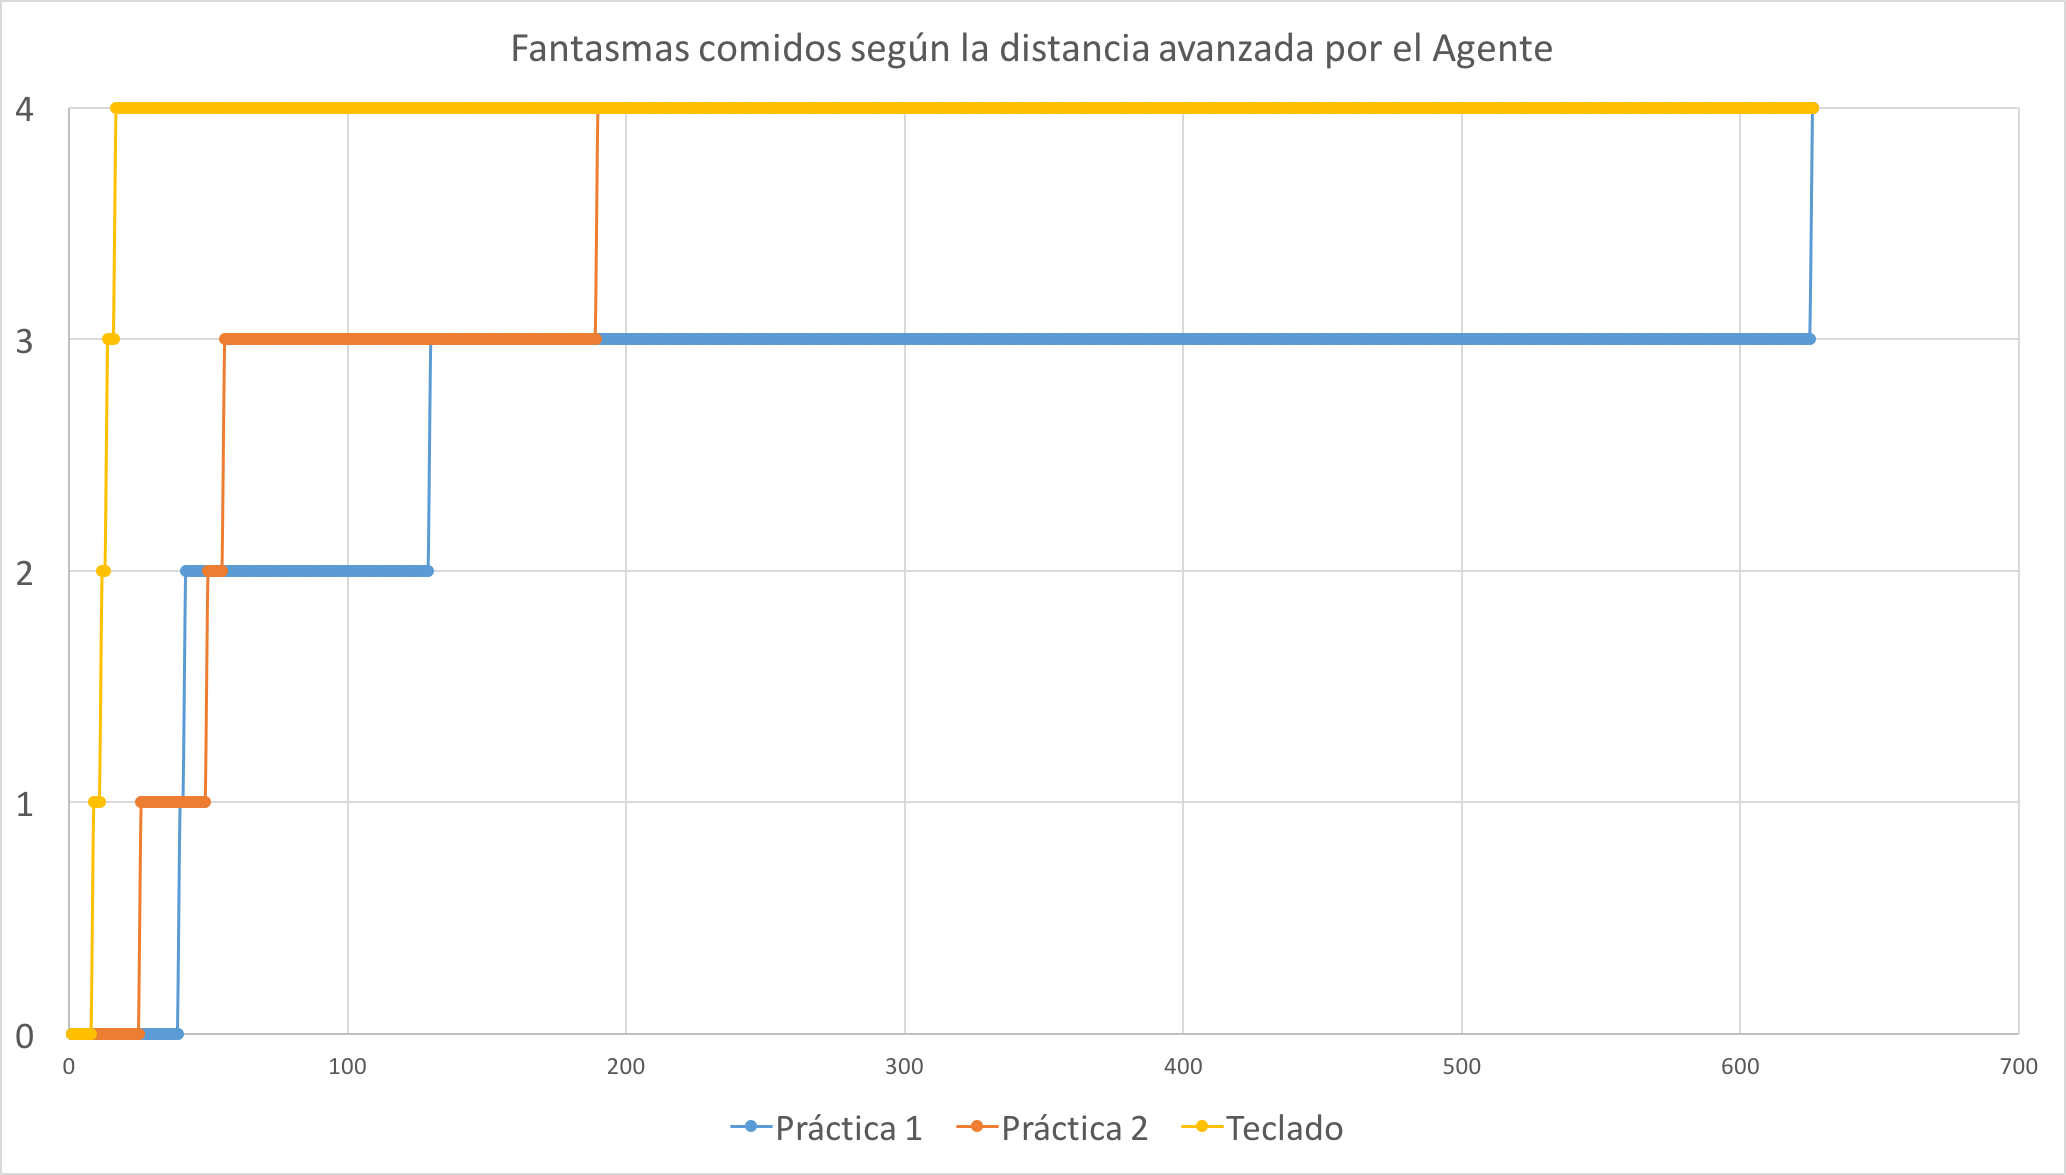
\includegraphics[width=15cm]{classicPerformanceComparison}
\end{center}

Si bien el agente de teclado (humano), al contar con la información extra de dónde está cada uno de los fantasmas en cada momento, es capaz de obtener un rendimiento bastante mejor (rozando el óptimo). Sin embargo, comparando los dos agentes automáticos observamos una \textbf{mejora muy clara} del nuevo agente respecto al anterior, de en torno al 60\%.
Sorprendidos con esta mejora tan llamativa, pasamos a comparar el tiempo empleado en cada turno para tomar la decisión que indicará a PacMan qué acción tomar. La siguiente gráfica compara el tiempo medio de respuesta de cada agente:

% TODO: la gráfica que está ahora compara sólo los <agente>classic.csv. Hacer una gráfica que contenga la media de cada uno de los agentes jugando varias partidas en 2 o 3 mapas de dimensiones parecidas (trickyClassic, openHunt y default)

\begin{center}
    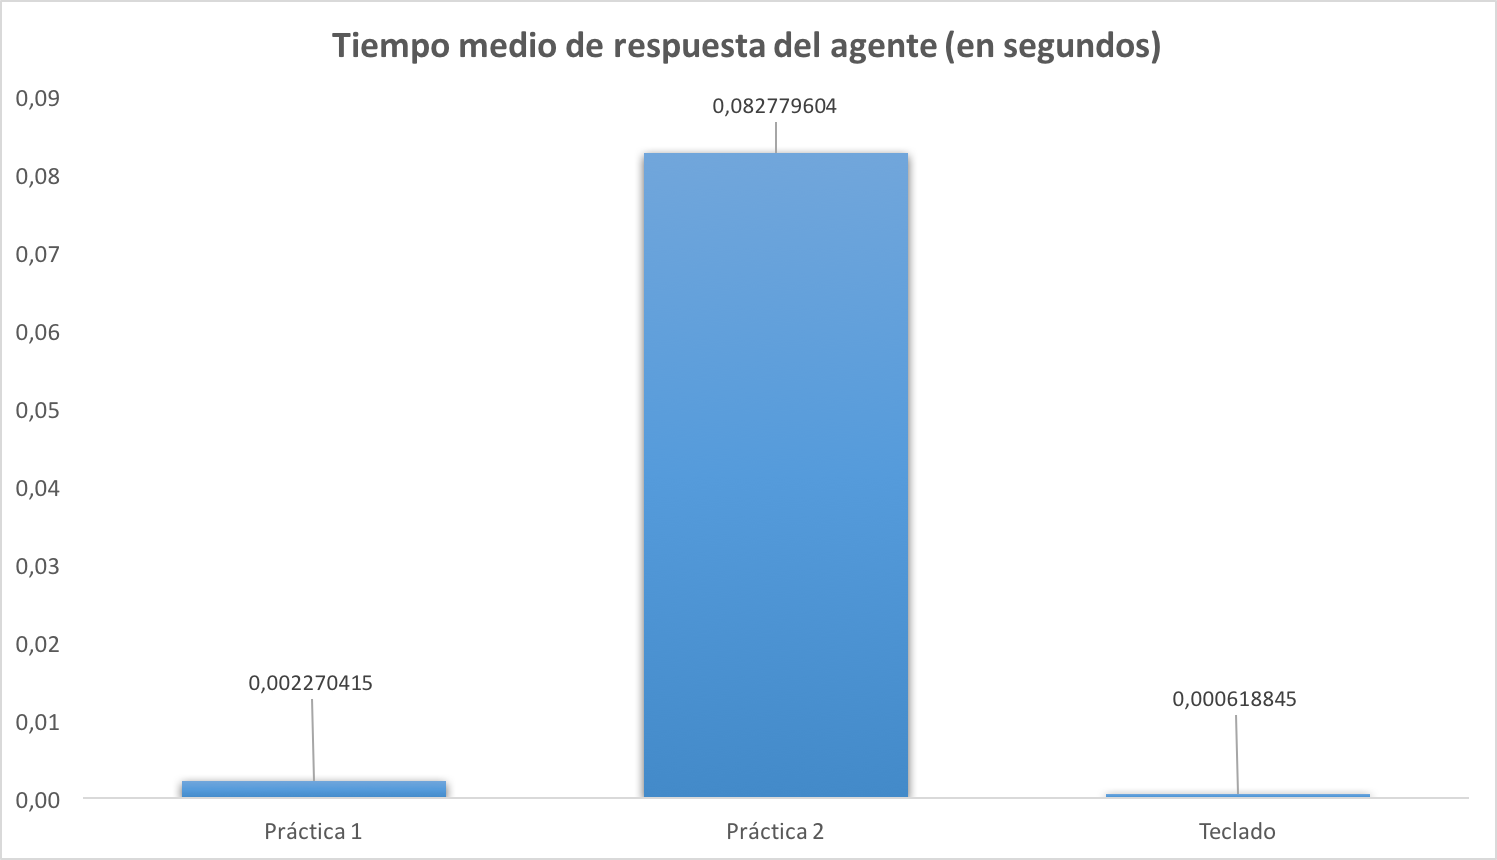
\includegraphics[width=15cm]{tiempoRespuesta}
\end{center}

Curiosamente, si bien el rendimiento comprobábamos que se había incrementado considerablemente con el agente que utiliza aprendizaje no supervisado, ahora observamos una \textbf{eficiencia mucho menor} en esta implementación. La causa de esta contrapartida es la cantidad de cómputo realizada por este agente en comparación con los otros dos:
\begin{itemize}
    \item El agente \textbf{humano} toma como tiempo de computación tan sólo lo que tarda el proceso de python en recibir e interpretar la tecla del teclado que ha pulsado el humano, siendo este un intervalo ínfimo, despreciable.
    \item El agente de la \textbf{Práctica 1} genera un árbol de clasificación al iniciar el juego con los datos que tenía antes de empezar una partida y, una vez generado, lo utiliza para clasificar cada nueva instancia. De esta forma, el tiempo real de cómputo se encuentra en la inicialización del agente, dejando para cada turno tan sólo el ``descenso'' del árbol de la nueva instancia que ``caerá'' en una clase o en otra.
    \item Sin embargo, el agente de esta \textbf{Práctica 2} compara, en cada turno, la nueva instancia con todas aquellas contenidas en el \emph{cluster} al que se le ha asignado. Esto requiere calcular la función de similitud por cada una de las instancias del clúster, lo que supone un tiempo muy elevado en cuanto a cómputo
\end{itemize}

% 4. Una tabla resumen con las medias y desviaciones estándar de los agentes en los distintos mapas.

% TODO: gráfica comparando los turnos que tarda cada agente en llegar a 4 fantasmas comidos según el mapa (jugar 3 partidas en cada mapa elegido, que yo creo que con 4 mapas distintos vale, con cada uno de los agentes y sacar la media de la duración de la partida)


\newpage
\section{Conclusiones}

El modelo obtenido en esta práctica puede ser útil como parte del agente automático para el juego de PacMan original, para la parte del juego en la que PacMan se ``come" una pieza de comida y comienza a perseguir a los fantasmas, y podría modificarse para reutilizarlo invirtiendo las funciones de forma que ``huyese" de ellos y buscase, en contraposición, las migas de pan que debe comerse.
Al realizar la práctica hemos entendido campos donde podrían usarse técnicas de aprendizaje automático como el cálculo de rutas en tiempo real para un vehículo que se mueve por un entorno, desde un coche que se mueve por las calles de una ciudad hasta una aeronave que se mueve entre vientos cósmicos.

\vspace{0.5cm}
\centerline{\textbf{Problemas encontrados}}
\vspace{0.5cm}

Como de costumbre en tareas de aprendizaje automático, los problemas surgidos durante el desarrollo de la \emph{práctica 2} han solido estar relacionados con los ``palos de ciego" necesarios para llegar a resultados concluyentes. bajo el lema de ``prueba, error y aprendizaje", el equipo trabajó para afinar los resultados tanto como fuese razonable.

\vspace{0.5cm}
\centerline{\textbf{Comentarios personales}}
\vspace{0.5cm}

Nos ha parecido muy interesante cómo la combinación de diferentes técnicas da como resultado una búsqueda más eficiente de soluciones, como en esta práctica el procesamiento de asociación en \emph{clusters} de los datos para reducir el dominio de búsqueda para la clasificación de una instancia. Este encuentro con el aprendizaje no supervisado nos ayudará a tener más herramientas a la hora de solucionar futuros problemas.

\end{document}
